%=================
\chapter{Sprint 3}
%=================


%------------------------
\section{Sprint Planning}
%------------------------
For the third sprint we intend to implement the remanding requirements in the product backlog. We feel that the first and second sprint has resulted in a satisfying utility, but it is still missing important functionality.

After two sprint iterations, we are still trying to improve our approach to Scrum. Each sprint results in new ideas and better ways to do the process, and in this sprint we want everything to be correct and in the right order.\\
\\
There will be two major changes this sprint:
\begin {itemize}
\item We will have a complete planning meeting. The meeting should result in a good planning document, user stories for all the requirements, complete set of work items in the sprint backlog and a early understanding of the design. This approach will be differently from earlier sprints, where user stories was written in parallel with implementation. The user story should now be in place before the implementation, and the implementation should be based on the user story. This will make documenting the process easier, and will in turn give the advisors more documentation of what we are doing. Then we can receive valuable feedback from them.

\item In the sprint backlog we will have work items for every task that needs to be done throughout the sprint, including writing minutes, doing documentation, implementation and so on.  Assignment of responsibilities for items in the backlog should not be done at the planning meeting, we rather only give responsibility for one item for each team member at a time. The rest of the items will be unassigned. At each stand-up meeting we pick a task and must be done before the next meeting. This will ensure efficiency and the work done by others are easier to check and revise. It will give us a better work balance, as no team member can gap over too many tasks and leave none for the others.
\end{itemize}
We think that these changes will improve our work efficiency, and make sprint 3 the best one so far.


\subsection{Duration}
%-----------------------

The sprint started with the planning meeting the 19th of October and our work started the following day. The sprint duration is 14 days, and will end the 1st of November with a review meeting. 


\subsection{Sprint Goal}
%-----------------------
For the third sprint the team will update CSjark to version 0.3 which will extend the utility so that it contains the complete functionality requested by the customer at this phase of the project. In this sprint we will pick all of the current requirements from the product backlog as all of the underlying functionality needed for them are already in place from the previous sprints. This means that we will also aim to create a draft of the final design of the system during the sprint.

The most important function that is going to be implemented in this sprint is being able to display packets from different originating platforms properly. This will be implemented by having every packet contain a flag specifying their originating platform, and by having our dissectors use this flag value to influence how it handles the data in the packet.

\subsection{Back Log}
%--------------------
The work items concering features for this sprint are covered by the user stories in the requirement section. <Make reference>
\\
See the timetable for sprint 3 in Table \ref{tab:sprint3time}.


\begin{table}[!htb] \small \center
\caption{Sprint 3 Timetable\label{tab:sprint3time}}
\begin{tabularx}{\textwidth}{X c c}
	\toprule
	& \multicolumn{2}{c}{Hours} \\
	\cmidrule(r){2-3}
	Description & Est. & Act. \\
	\midrule
	\textbf{Sprint planning} & \textbf{30} & \textbf{47.5} \\
	\addlinespace
	\textbf{Sprint 3 requirements} & \textbf{102} & \textbf{-} \\
	Implementation & 72 & - \\
	Testing & 19 & - \\
	User Documentation & 11 & - \\
	\addlinespace
	\textbf{Sprint review} & \textbf{20} & \textbf{-} \\
	\addlinespace
	\textbf{Sprint documentation} & \textbf{75} & \textbf{-} \\
	Sprint 1 document & 10 & -\\
	Sprint 2 document & 14 & - \\
	Sprint 3 document & 51 & - \\
	\addlinespace
	\textbf{Report work} & \textbf{42} & \textbf{-} \\
	User stories to LaTeX & 3 & 4\\
	Architecture update & 8 & -\\
	Glossaries and acronyms & 16 & -\\
	Requirement review & 15 & -\\
	Layout and correction & 15 & -\\
	\addlinespace
	\textbf{Lectures} & \textbf{21} & \textbf{14} \\
	\addlinespace
	\textbf{Meetings} & \textbf{57} & \textbf{-} \\
	Advisor meetings & 28 & - \\
	Customer meetings & 8 & - \\
	Stand-up meetings & 21 & - \\
	\midrule
	Total: & 347 & - \\
	\bottomrule
\end{tabularx}
\end{table}



%----------------------
\section{System Design}
%----------------------


%-----------------------
\section{Implementation}
%-----------------------
The main focus for this sprint was to support of different platforms. Several 
things are dependent on platform; endianness, the memory allingment and sizes 
of data types. It is also possible that structs can be defined differnt for 
each platform. The utility will generate different dissectors for each 
platform. A dissector this wil detect the platform and use the correct 
platform dissector.

Support for the union data type, finishing implementation of custom Lua files 
and modification of functionallity implemented in the previous sprint was also 
done in this sprint.

\subsection{Specify Flags for Each Platform}
%-----------------------
It is necessary to specify flags for each platform to make it possible to 
correctly detect and display packages that wireshark captures. In wireshark 
the flags are used to tell which platform the package is sent from, so that 
the right dissector is used to display the package in Wireshark. In the 
utility the flag points to what kind of endianness, how memory is aligned and 
the different sizes that is used for data types on the platform. These data 
are used to genereate a dissector for the specific platform.

\subsection{Support Little and Big Endian}
%-----------------------
Different platforms can order bytes in either little(left-to-right) or 
big(right-to-left) endian. The Windows platform uses little endian, and SPARC 
uses big endian. Since the utility has to support both platforms, it was 
necessary to support handling of endianness. The Lua API in wireshark has 
functionallity to display data in both little and big endian. Therefore the 
utility has to read the specfied flag for the platform, and generate a Lua 
dissector that displays the data correctly for the given platform.

\subsection{Support Different Sizes from Flags}
%-----------------------
TODO

\subsection{Support Platform Specific Macros}
%-----------------------
TODO

\subsection{Support Custom Lua Files}
%-----------------------
TODO

\subsection{Support Wireshark Filter and Search}
%-----------------------
TODO

\subsection{Support Different Memory Alignment}
%-----------------------
TODO

\subsection{Support Union Type}
%-----------------------
\autoref{fig:wsunion}

\begin{figure}[ht]
	\center
	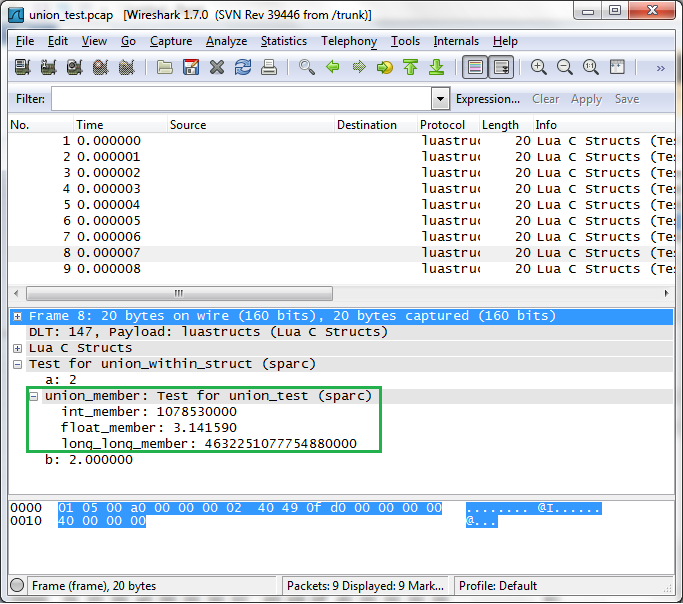
\includegraphics[width=\textwidth]{./sprints/img/wireshark_union}
	\caption{Union type support\label{fig:wsunion}}
\end{figure}

%\lstset{language=C,caption={Struct for custom handling},label=code:customstruct}
%\lstinputlisting[language=C]{./sprints/code/customfield.h}

TODO

\subsection{Display Types Wireshark Do Not Support}
%-----------------------
TODO

\subsection{Support Specifying ID of Dissectors}
%-----------------------
TODO

\subsection{Do Not Regenerate dissectors}
%-----------------------
TODO

\subsection{Handle Lua Reserved Keywords}
%-----------------------
Lua has a list of reserved keywords, and some of these keywords are allowed in 
the C language. The utility is able to support this under generation of Lua 
code, when an identifier is a lua keyword, an underscore(\_) is added, so the 
identifier start with ''\_''.

%-----------------------
\section{Sprint Testing}
%-----------------------


%--------------------------
\section{Customer Feedback}
%--------------------------


%--------------------------
\section{Sprint Evaluation}
%--------------------------


